\section{moGenSolContinue$<$ EOT $>$ Class Template Reference}
\label{classmo_gen_sol_continue}\index{moGenSolContinue@{moGenSolContinue}}
One possible stopping criterion for a solution-based heuristic.  


{\tt \#include $<$moGenSolContinue.h$>$}

Inheritance diagram for moGenSolContinue$<$ EOT $>$::\begin{figure}[H]
\begin{center}
\leavevmode
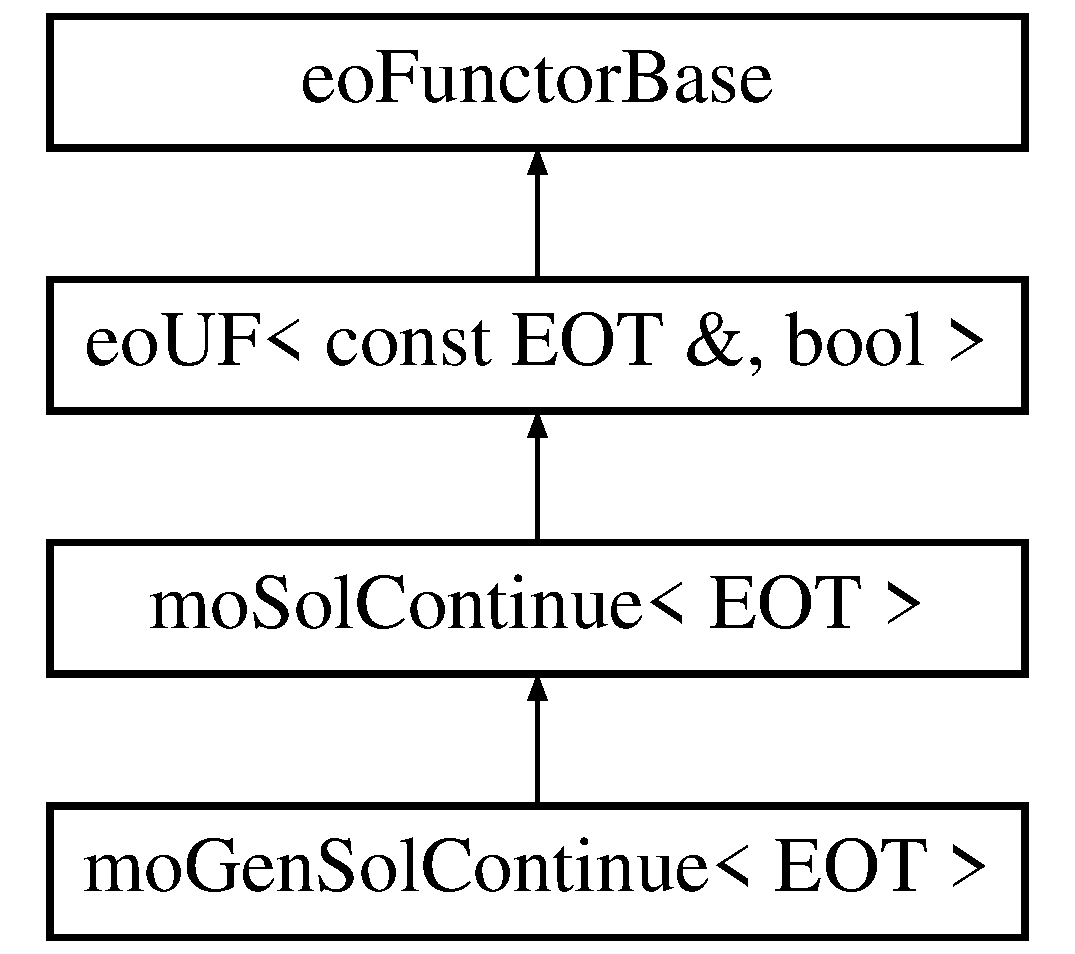
\includegraphics[height=4cm]{classmo_gen_sol_continue}
\end{center}
\end{figure}
\subsection*{Public Member Functions}
\begin{CompactItemize}
\item 
{\bf moGenSolContinue} (unsigned int \_\-\_\-maxNumGen)
\begin{CompactList}\small\item\em Basic constructor. \item\end{CompactList}\item 
bool {\bf operator()} (const EOT \&\_\-\_\-sol)
\begin{CompactList}\small\item\em Function that activates the stop criterion. \item\end{CompactList}\item 
void {\bf init} ()\label{classmo_gen_sol_continue_6c5db8182157584b56507cc9075602d4}

\begin{CompactList}\small\item\em Procedure which allows to initialise all the stuff needed. \item\end{CompactList}\end{CompactItemize}
\subsection*{Private Attributes}
\begin{CompactItemize}
\item 
unsigned int {\bf maxNumGen}\label{classmo_gen_sol_continue_30b9861e090578bdfa2374806600987a}

\begin{CompactList}\small\item\em Iteration maximum number. \item\end{CompactList}\item 
unsigned int {\bf numGen}\label{classmo_gen_sol_continue_630d9736a3a2c952540cdc211764258c}

\begin{CompactList}\small\item\em Iteration current number. \item\end{CompactList}\end{CompactItemize}


\subsection{Detailed Description}
\subsubsection*{template$<$class EOT$>$ class moGenSolContinue$<$ EOT $>$}

One possible stopping criterion for a solution-based heuristic. 

The stopping criterion corresponds to a maximum number of iteration. 



Definition at line 21 of file moGenSolContinue.h.

\subsection{Constructor \& Destructor Documentation}
\index{moGenSolContinue@{moGenSolContinue}!moGenSolContinue@{moGenSolContinue}}
\index{moGenSolContinue@{moGenSolContinue}!moGenSolContinue@{moGenSolContinue}}
\subsubsection{\setlength{\rightskip}{0pt plus 5cm}template$<$class EOT$>$ {\bf moGenSolContinue}$<$ EOT $>$::{\bf moGenSolContinue} (unsigned int {\em \_\-\_\-maxNumGen})\hspace{0.3cm}{\tt  [inline]}}\label{classmo_gen_sol_continue_b56e890f1caa3f98e161c6512b59c95b}


Basic constructor. 

\begin{Desc}
\item[Parameters:]
\begin{description}
\item[{\em \_\-\_\-maxNumGen}]the maximum number of generation. \end{description}
\end{Desc}


Definition at line 30 of file moGenSolContinue.h.

\subsection{Member Function Documentation}
\index{moGenSolContinue@{moGenSolContinue}!operator()@{operator()}}
\index{operator()@{operator()}!moGenSolContinue@{moGenSolContinue}}
\subsubsection{\setlength{\rightskip}{0pt plus 5cm}template$<$class EOT$>$ bool {\bf moGenSolContinue}$<$ EOT $>$::operator() (const EOT \& {\em \_\-\_\-sol})\hspace{0.3cm}{\tt  [inline, virtual]}}\label{classmo_gen_sol_continue_457257cd73b474d6f7783d84d02c2e61}


Function that activates the stop criterion. 

Increments the counter and returns true if the current number of iteration is lower than the given maximum number of iterations.

\begin{Desc}
\item[Parameters:]
\begin{description}
\item[{\em \_\-\_\-sol}]the current solution. \end{description}
\end{Desc}
\begin{Desc}
\item[Returns:]true or false according to the current generation number. \end{Desc}


Implements {\bf eoUF$<$ const EOT \&, bool $>$}.

Definition at line 42 of file moGenSolContinue.h.

References moGenSolContinue$<$ EOT $>$::maxNumGen, and moGenSolContinue$<$ EOT $>$::numGen.

The documentation for this class was generated from the following file:\begin{CompactItemize}
\item 
moGenSolContinue.h\end{CompactItemize}
